\chapter{Cats}

I do not usually talk about myself, but when I do, I talk about my cat.\\

In April 2010, the American economy was gripped by its most severe economic crisis in at least a generation.  There was in a deep recession.  It was in this climate that a great savior was born; her name is Muffins.  

\begin{figure}[ht!]
\centering
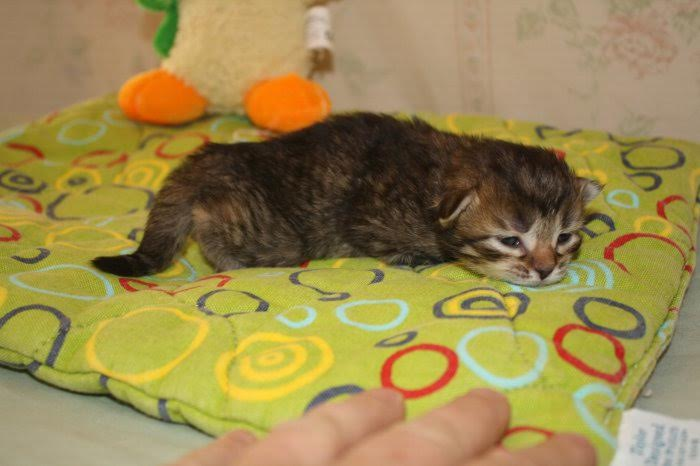
\includegraphics[width=90mm]{./images/muffins.jpg}
\caption{A Week Old Muffins}
\end{figure}

She is the first cat I have ever owned.  She is a purebred Siberian.  Her interests include: \\
\begin{itemize}
	\item Sleeping
	\item Grooming herself
	\item Twister
\end{itemize}

The reason I chose to get a Siberian cat is because they are purported (perhaps dubiously) to be hypoallergenic. They are also a very healthy breed as they were more recently domesticated.\

\section{Career Goals}

I am impressed by the ground working done by the renowned dog rehabilitator Cesar Millan, host of the critically acclaimed television show "Dog Whisperer." It is my hope that I could have an equally successful television program which I will entail "Cat Telepathist"  where I will rehabilitate troubled and stray cats through the power of extrasensory perception (ESP).

If my "Cat Telepathist" show were not to find a niche with audiences, my second television show is modeled after the former television show "Crossing Over with John Edward." \cite{calderwood} I plan to call the show "You have Cat to be Kitten Me with Zayd Hammoudeh" and will be used to give grieving families the opportunity to communicate with their deceased feline family members.

Other TV show ideas I would like to pursue include:
\begin{itemize}
	\item Cat Mustache Aficionado - A daily discussion of cat whiskers.
	\item Alien vs. Predator vs. Cat - It is like the movie "Alien vs. Predator" but instead of it being a two party battle, it is a triple threat match with a cat.
	\item Cat Hoarders - A show where we do an intervention with a cat that hoards some type of item.
\end{itemize}